% Первая глава работы 
\chapter{Название главы}
\label{chap1}

\section{Название секции}
\label{chap1:sec1}

% Пример оформления списка
% 
Фильтрующий маршрутизатор фильтрует IP-пакеты на основе групп
следующих полей заголовка пакета:

\begin{itemize}
\item IP-адрес отправителя;
\item IP-адрес получателя;
\item порт отправителя;
\item порт получателя.
\end{itemize}

На всю литературу надо ссылаться~\cite{medvedovsky:1997:ataka, romanets:security}.

\section{Название секции}
\label{chap1:sec2}

% Примеры оформления рисунков
%
На рисунке~\ref{fig1} представлена упрощенная схема построения современного МЦОВ.

\begin{figure}
 \centerline{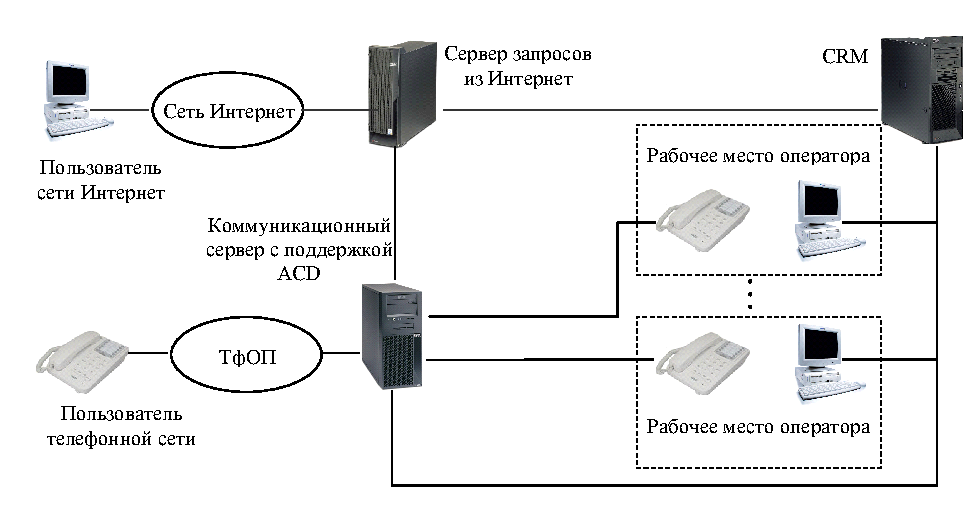
\includegraphics[width=0.7\textwidth]{fig1}}
 \caption{Упрощённая схема построения МЦОВ}
\label{fig1}
\end{figure}

На рисунке~\ref{fig4} представлен граф интенсивностей переходов для рассматриваемой СМО с параметрами \(c = 2\) и \(r = 3\).

\begin{figure}
 \centerline{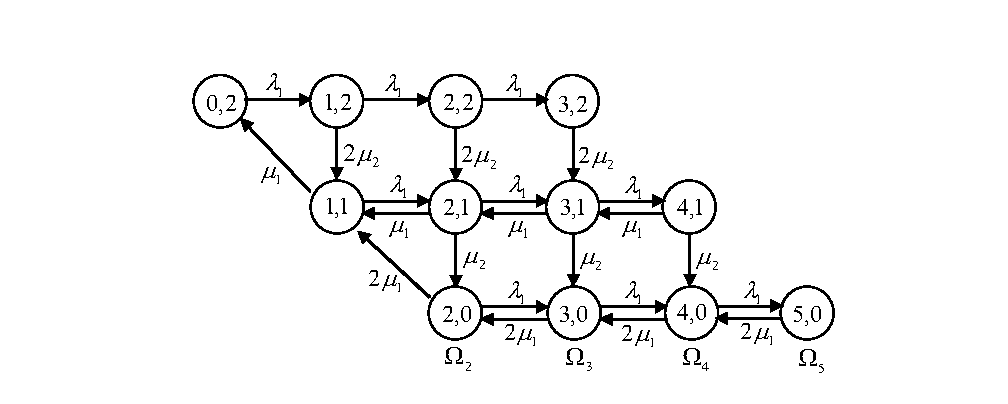
\includegraphics[width=0.9\textwidth]{fig4}}
 \caption{Граф интенсивностей переходов}
\label{fig4}
\end{figure}

На рис.~\ref{fig6} представлены графики зависимости \(\pi _1\) от \(\rho _1\) для различных \(\mu _2\).

\begin{figure}
\centerline{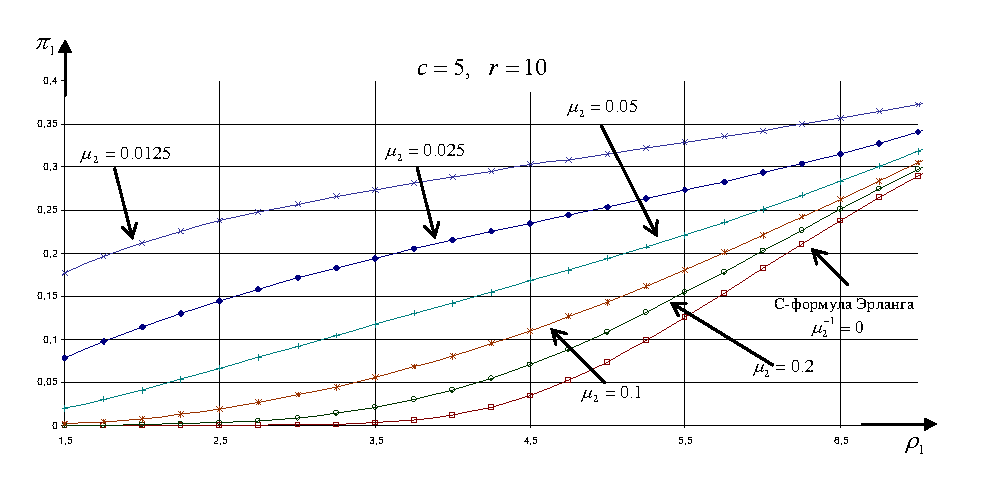
\includegraphics[width=0.9\textwidth]{fig6}}
\caption{Зависимость \(\pi _1\) от \(\rho _1\) для различных \(\mu _2\)}
\label{fig6}
\end{figure}

%%


\section{Название секции}
\label{chap1:sec3}

Введём два случайных процесса \(X_1 (t)\)~--- суммарное количество 1-вызовов на приборах и в накопителе, \(X_2 (t)\)~--- количество 2-вызовов на приборах в момент времени \(t\), \(X_1 (t) = \overline {0,R} \), \(X_2 (t) = \overline {0,c} \), \(X_\bullet (t) = \overline {c,R} \). Тогда функционирование системы может быть описано ступенчатым Марковским процессом \(\overrightarrow X (t) = (X_1 (t),X_2 (t))\) со следующим пространством состояний:
\begin{equation}
\label{eq:01}
\Omega = \coprod\limits_{\alpha = c}^R \Omega _\alpha , \quad
\Omega _\alpha = \left\{ {(i,j):i + j = \alpha }\right\}, \quad
\alpha = \overline {c,R}.
\end{equation}

%%% Local Variables:
%%% mode: latex
%%% coding: utf-8-unix
%%% End:
